\documentclass[12pt]{article}

\usepackage[utf8]{inputenc}
\usepackage[portuguese]{babel}
\usepackage{indentfirst}
\usepackage{amsmath}
\usepackage{hyperref}
\usepackage[numbers,super]{natbib}
\usepackage{graphicx}
\usepackage{geometry}

\geometry{
	paper = a4paper,
    inner = 3cm,
    outer = 3cm,
    bindingoffset = .5cm,
    top = 2cm,
    bottom = 2cm
}

\begin{document}

% Title page
\begin{titlepage}
\begin{center}

%%% ACF Evite formatar à força. Procure algum estilo que lhe agrade
\textbf{\LARGE Universidade Federal de Alagoas } \\[0.5cm]
\textbf{\large Instituto de Computação - IC}\\[0.2cm]

\vspace{20pt}

\vspace{20pt}
\vspace{20pt}
\vspace{20pt}
\vspace{20pt}
\vspace{20pt}
\vspace{20pt}
\vspace{20pt}
\vspace{20pt}

\textbf{\Large Aluno: Danilo Fernandes Costa}\\
\vspace{70pt}
\textbf{\LARGE Relatório de acopanhamento de pesquisa}\\
\vspace{20pt}
\textbf{\Large Análise e processamento de imagens PolSAR}\\
\vspace{70pt}
\textbf{\large Orientador: Alejandro Frery}\\

\vspace{45pt}
\end{center}

\par
\vfill
\begin{center}
\textbf{Maceió - AL}\\
\textbf{2018}
\end{center}

\end{titlepage}

\newpage

\section{Resumo}

No presente relatório são apresentados os histogramas referentes aos dados de cada uma das bandas de uma região homogênea extraída de uma imagem PolSAR. 
Além disso, tal imagem é o resultado da aplicação de um filtro baseado no coeficiente de variação às bandas de intensidade da imagem original.  

Para avaliar a adesão desses dados ao modelo gama, foram estimados os parâmetros dos mesmos para esse modelo e, a partir destes, obtida a função de densidade de probabilidade. 
A estimação dos parâmetros foi feita através do método de Máxima Verossimilhança, o qual encontra-se implementado pela biblioteca \texttt{stats4}.

\section{Estimação por Máxima Verossimelhança}

Sejam $X_1, \dots, X_n$ variáveis aleatórias que constituem uma amostra aleatória de uma distribuição discreta ou contínua cuja função de probabilidade ou função de densidade de probabilidade é $f(x\mid \theta)$, onde o vetor de parâmetros $\theta$ pertence a um certo espaço paramétrico $\Omega$. 

Para cada observação \textbf{x} = $(x_1, \dots, x_n)$ da amostra, denotemos por $f_n(\textbf{x}\mid \theta)$ o seu respectivo valor da função de probabilidade conjunta ou função de densidade de probabilidade conjunta. 
Desse modo, se tomarmos $f_n(\textbf{x}|\theta)$ como uma função de $\theta$ para dados valores de $x_1,\dots, x_n$, passamos a chamá-la de função de verossimilhança.

Em posse disso, se denotarmos por $\delta(\textbf{x})$ como o valor de $\theta$ que maximiza a função de verossimilhança $f_n(\textbf{x}\mid\theta)$ para uma dada observação $\textbf{x} = (x_1, \dots, x_n)$ da amostra, podemos definir $\widehat{\theta} = \delta(\textbf{X})$ como o estimador de $\theta$. 
%%% ACF: é estimador quando depende de variáveis aleatórias; quando depende de observações, é estimativa.
Esse e $\delta(\textbf{x})$ são chamados estimador e estimativa de máxima verossimelhança de $\theta$, respectivamente.

Dessa forma, o problema de estimação de parâmetros torna-se um problema de maximização de uma função. 
Todavia, uma abordagem relevante é transformá-lo em uma minimização de $g_n(\textbf{x}|\theta) = -\log(f_n(\textbf{x}|\theta))$, visto que $X_1,\dots, X_n$ são independentes e, portanto: 
%%% ACF O fato de serem independentes redunda no produto. Maximizar o logaritmo é possível porque são funções de probabilidade e, com isso, sempre positivas
%%% ACF Revise a notação daqui em diante
\begin{displaymath}
g_n(\textbf{x}|\theta) = -log( f_n(x_1, ..., x_n|\theta) ) = -log( \prod_{i = 1}^{n} f(x_i|\theta) ) = - \sum_{i = 1}^{n} log( f(x_i|\theta) ),
\end{displaymath}
%%% ACF Nunca deixe linha em branco antes de algo que dá continuidade ao parágrafo
onde $g_n(\textbf{x}|\theta)$ é chamada função de log-verossimelhança negativa.

\section{Análise de imagens PolSAR}

A região escolhida para realização da análise corresponde à matriz de 90 x 95 (pixels) contida no retângulo de arestas brancas na imagem abaixo:

\begin{figure}[hbt]
    \centering
    %%% ACF Prefira estipular o tamanho das figuras em termos da proporção da largura da linha: .6\linewidth
    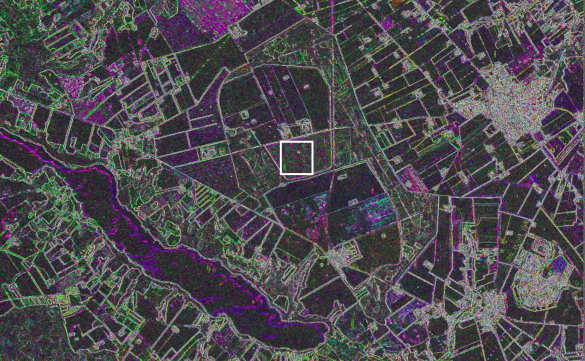
\includegraphics[scale = 0.65]{../../Images/Report_18_09_17/region.png}
\end{figure}

Para estimativa dos parâmetros da distribuição gama, os quais são \textit{forma} e \textit{média}, utilizou-se o código abaixo. 
Neste, \texttt{NegLogLik} consiste na função de log-verossimelhança negativa a ser otimizada e \texttt{mle} (\textit{Maximum Likelihood Estimation}) é a função que realiza tal processo, a qual é provida pela biblioteca \texttt{stats4} e recebe uma função, os parâmetros iniciais e um método para a otimização.

%%% ACF Use algum estilo LaTeX adequado para código
\begin{verbatim}
NegLogLik <- function(alpha, beta) {
  -sum(dgamma(vector_data, shape = alpha, rate = beta, log=TRUE))
}

MLE.fit = mle(minuslogl = NegLogLik, start = list(alpha = 1, beta=1), 
                method = "Nelder-Mead")

summary(MLE.fit)
\end{verbatim}

%%% ACF Diga explicitamente quais são os resultados: figuras, tabelas etc.
Seguem os resultados

%%% Use o pacote subfig
\begin{figure}[hbt]
    \centering
    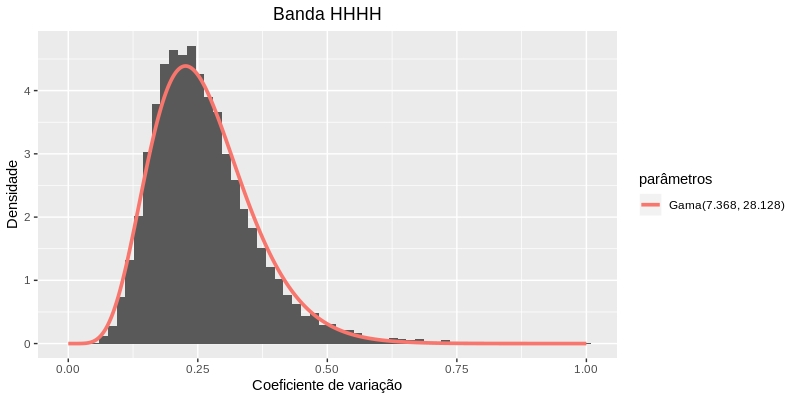
\includegraphics[scale = 0.75]{../../Images/Report_18_09_17/density_hhhh.jpeg}
\end{figure}

\begin{figure}[!ht]
    \centering
    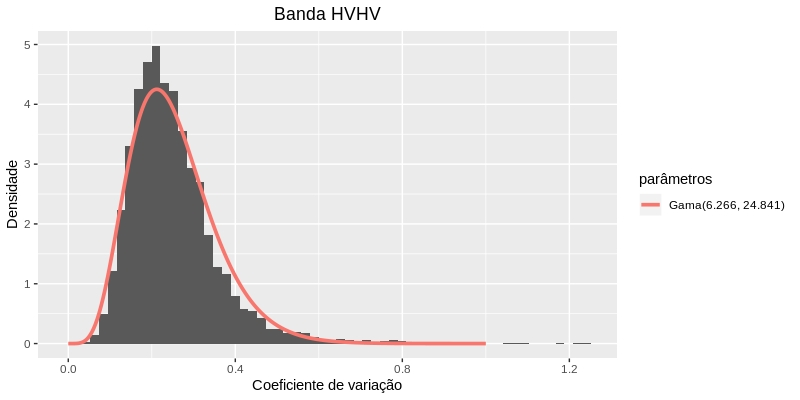
\includegraphics[scale = 0.75]{../../Images/Report_18_09_17/density_hvhv.jpeg}
\end{figure}

\begin{figure}[!ht]
    \centering
    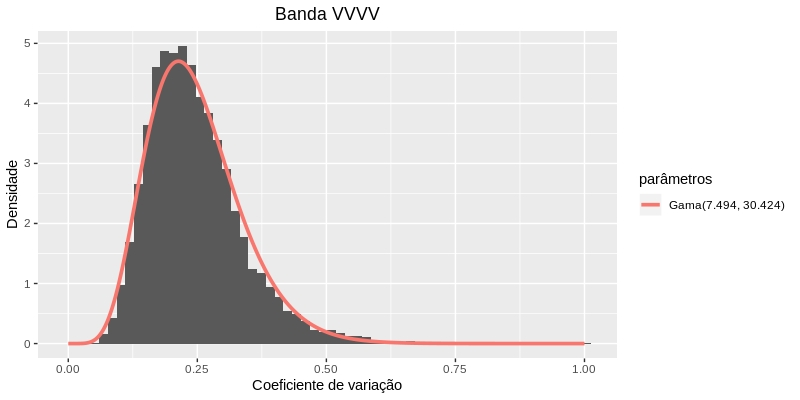
\includegraphics[scale = 0.75]{../../Images/Report_18_09_17/density_vvvv.jpeg}
\end{figure}

%%% ACF Comente os resultados. Além do visual, consegue imaginar como avaliar o ajuste?

\end{document}
